\graphicspath{{./Figs/}}

\chapter{Introduction} 
\label{sec:Background}

% What is a MAV

% These advances have largely been brought about by technological advances in power processors, miniature sensors, and control theory \cite{NONAMI2007}.


Unmanned aerial vehicles (\acrshort{UAV}s) are used throughout various industries to conduct missions that are either dangerous, difficult or dull for humans to perform. Recently \acrshort{UAV}s have seen unprecedented growth for both commercial \cite{Liu2014} and military \cite{Chaturvedi2019, Fan2018} use. The capability to fly within narrow spaces gives Micro Aerial Vehicles (\acrshort{MAV}s) a significant advantage over general \acrshort{UAV}s in specific use cases. \acrshort{MAV}s, in particular, are more manoeuvrable in cluttered environments, such as, collapsed buildings, commercial centres, and search and rescue missions. Given current technology, \acrshort{MAV}s could provide coordinates of trapped victims in areas where it would be dangerous to search manually \cite{Valavanis2007}. Possible applications of \acrshort{MAV}s include dangerous gas detection, environmental monitoring, border patrol, mapping, precision agriculture, homeland security, and drug interdiction \cite{Liu2014, Valavanis2007}. \acrshort{MAV}s ability to be much quieter and concealed give it a major advantage over \acrshort{UAV}s \cite{Chaturvedi2019}.


Today defence programs around the world utilize \acrshort{UAV}s for reconnaissance, surveillance, damage assessments, and communication relay \cite{Chaturvedi2019, Fan2018, Valavanis2007}. \acrshort{MAV}s have even more recently seen major research interest, particularly in the last decade \cite{Valavanis2007}.  The relative size of \acrshort{MAV}s to other typical aircraft is shown in Figure \ref{fig:sizes}. Smaller vehicles are intended to lower the total cost of systems currently used and increase the portability of \acrshort{MAV}s \cite{Stephen2022}. The most significant factors for \acrshort{MAV} design, are current limitations in propulsion, configuration, and flight control \cite{Stephen2022}.


\begin{figure}[H]
  \centering
%   \hspace*{-0.4cm}
   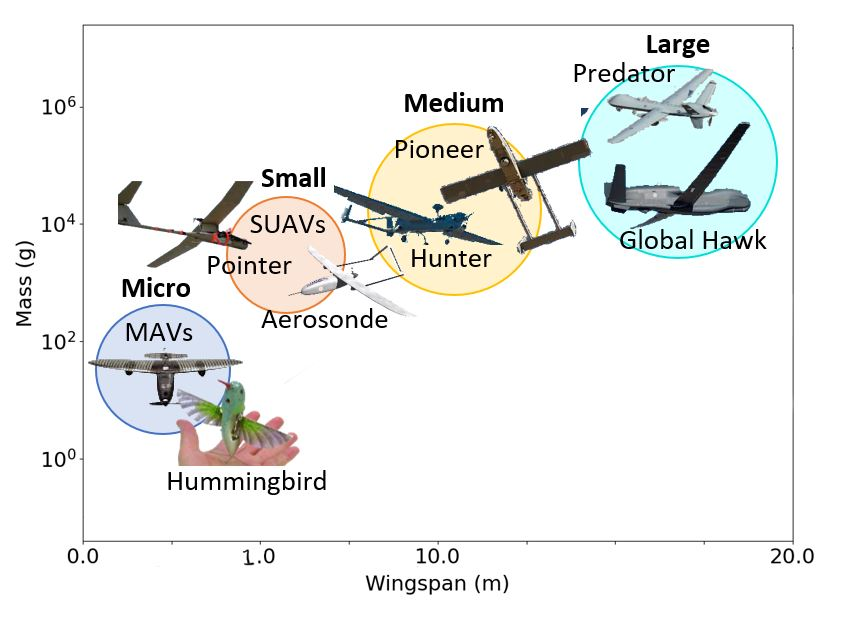
\includegraphics[width=\linewidth]{01_Introduction/Figs/replacement.JPG}
  \caption{\acrshort{MAV} gross weight with wing span. Figure is adapted \cite{uavsize}. Image sources: \cite{MAVImage, Hummingbird, Ava, Aerosonde, hunter, pioneer, MQ9, hawk}}
  \label{fig:sizes}
\end{figure}


\acrshort{MAV}s fall into three main categories. These are fixed wings \cite{Stanford2008}, rotary wings \cite{Lasek2001} and flapping wings \cite{Platzer2012}, which can also be used in combination.







\begin{figure}[H]
     \centering
     \begin{subfigure}[b]{0.3\textwidth}
         \centering
         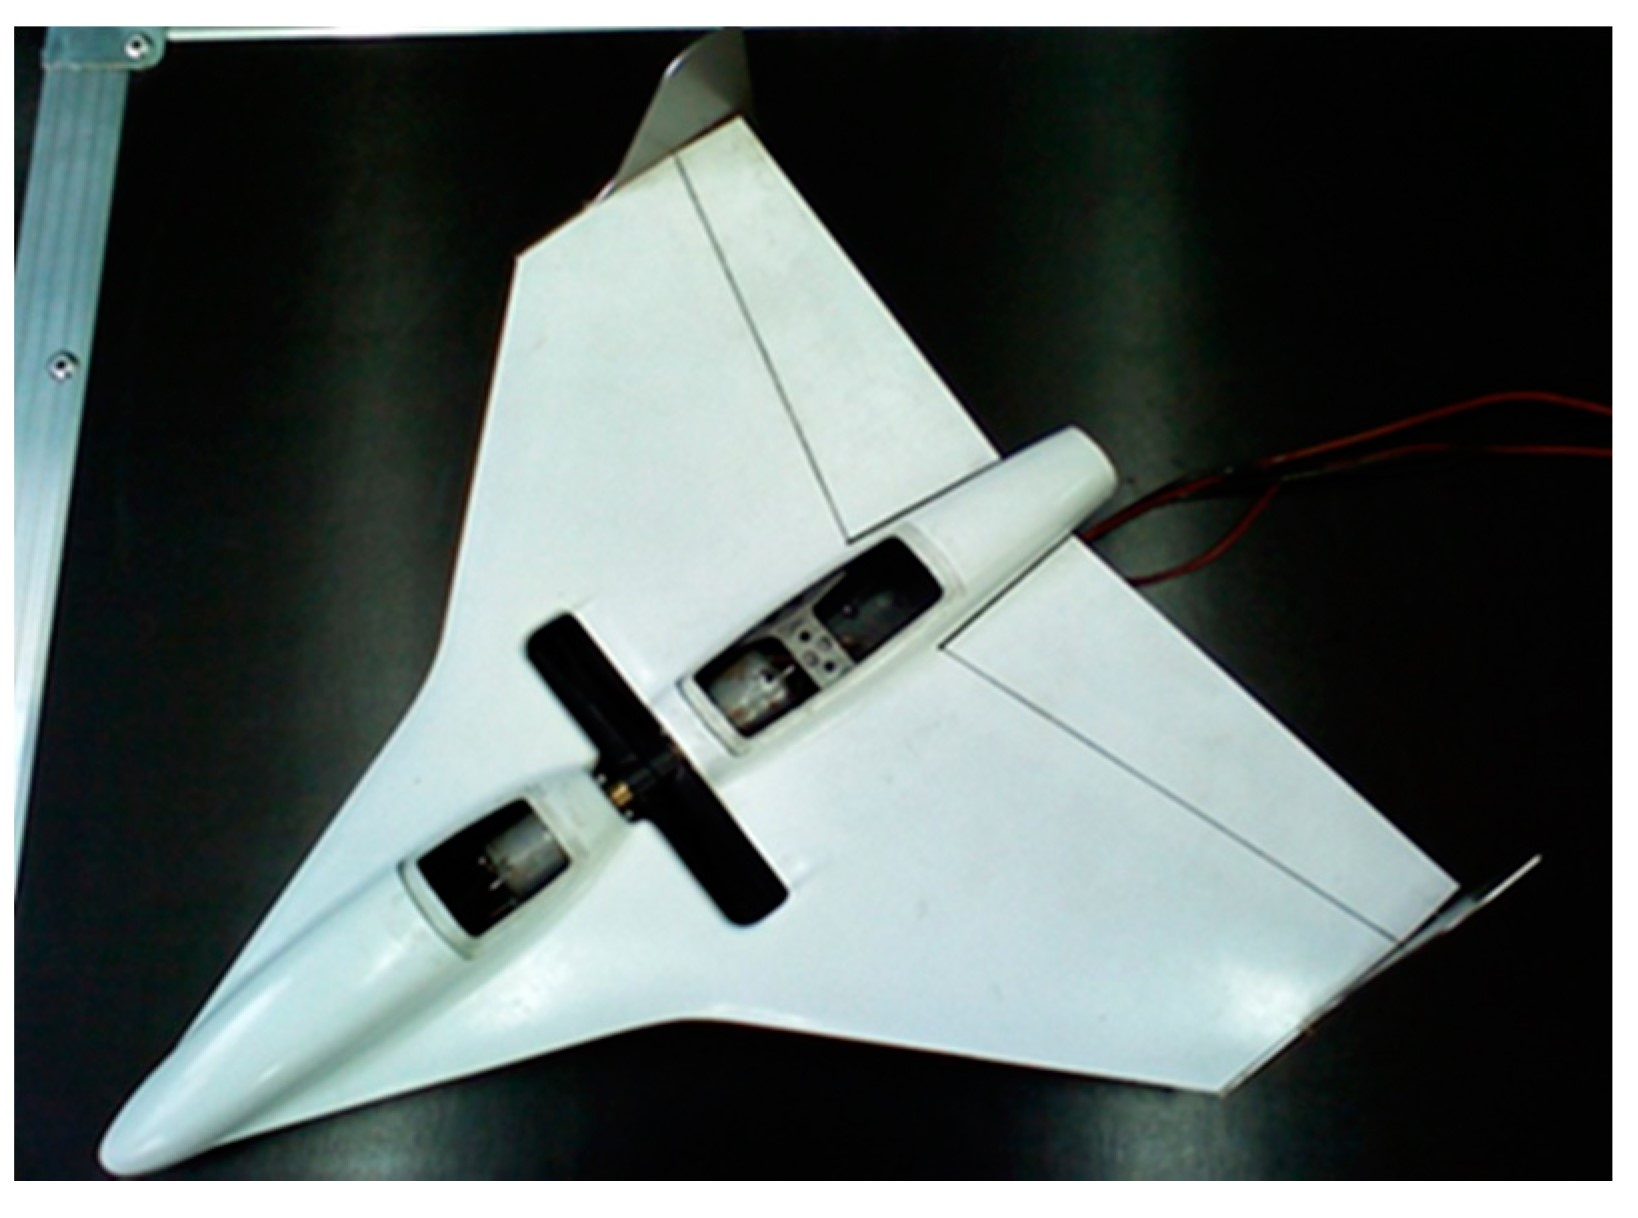
\includegraphics[width=\textwidth]{01_Introduction/Figs/fixed.jpg}
         \caption{Fixed wing \acrshort{MAV} \cite{Sibilski2020}}
         %\label{fig:y equals x}
     \end{subfigure}
     \hfill
     \begin{subfigure}[b]{0.3\textwidth}
         \centering
         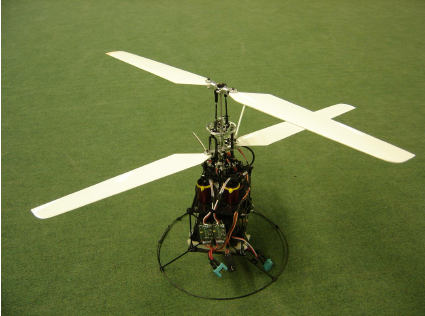
\includegraphics[width=\textwidth]{01_Introduction/Figs/rotar.png}
         \caption{Rotor \acrshort{MAV} \cite{rotar2022}}
         %\label{fig:three sin x}
     \end{subfigure}
     \hfill
     \begin{subfigure}[b]{0.3\textwidth}
         \centering
         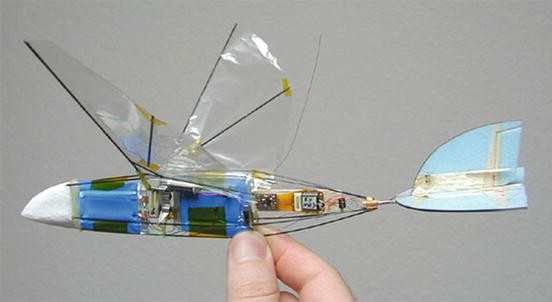
\includegraphics[width=\textwidth]{01_Introduction/Figs/flapping.jpg}
         \caption{Flapping wing \acrshort{MAV} \cite{Jones2015}}
         %\label{fig:five over x}
     \end{subfigure}
        \caption{Examples of \acrshort{MAV}s with category}
        \label{fig:threeDesigns}
\end{figure}


\acrshort{MAV}s are much more difficult to design and manufacture than typical aircraft  \cite{Ward2017}. This additional complexity is due to several factors:
\begin{itemize}
  \item Low speed flight
  \item Small physical dimensions
  \item Structural strength
  \item Reduced stall speed due to smaller size
  \item Low inertia
\end{itemize}



% \\
With the increased complexity of \acrshort{MAV} designs, there has also been an increased interest in the research and design of optimised \acrshort{MAV} models \cite{Ward2017}. Design software to optimise \acrshort{MAV} designs is generally based on aerodynamic properties, weights, stability, and maneuverability \cite{Amadori2012, Vijayanandh2019, Radmanesh2014}. The low-speed and non-linear flight dynamics are of particular importance for \acrshort{MAV} development \cite{Aboelezz2020, Aboelezz2021}. The low speeds that \acrshort{MAV}s fly at and the influence of an operating propeller on the rest of the \acrshort{MAV} is currently unvalidated with physical wind tunnel testing. This thesis aims to fill in this gap.

% There is no physically validated MAV modelling  validated, reliable optimisation technique for MAV aircraft design.

% 

% Intro here




\section{Problem Statement}
\label{ProblemStatement}

In the past, surveillance was conducted initially from hot air balloons. Later, aircraft such as helicopters would be used, costing companies large sums of money to survey from a bird's eye view \cite{Aleksander2018}. Today drones and \acrshort{UAV}s often conduct this work, within certain limits due to range and flight time \cite{NONAMI2007, Aleksander2018}. The next significant technology jump sees the optimisation and miniaturisation of these aircraft to produce \acrshort{MAV}s. \acrshort{MAV}s are set to increase the ability to conduct a variety of missions that predominately have military or surveillance objectives \cite{Aleksander2018, Mil2022, Greenwood2019, Saytov2022}. 

The \acrshort{MAV}'s main deferring attributes are; its smaller size, lower radar visibility and lower noise output. With \acrshort{MAV} design becoming one of the fastest-growing areas of development in the aerospace industry, there is an increasing need to have accurate experimental data to validate, simulate and model the numerous \acrshort{MAV} configurations being investigated. One of the core but currently missing pieces to this puzzle is the influence and effect of propellers on the aerodynamics and stability of \acrshort{MAV}s. Can we further deepen our understanding of \acrshort{MAV}s by analysing these effects?
% DEEPERRR

% paragraph on impact\significance of MAV
% MAV's

% paragraph on current Limitations


% paragraph on challenge/ main goal 
\section{Objectives}
\label{sec:Objectives}
The objectives of this thesis are as follows:

\begin{enumerate}
   \item To review current published literature and determine areas with insufficient or no research available for further development and research.
  \item To design and produce a 3D model of a \acrshort{MAV} with a detachable propeller to allow for both tractor and pusher configurations.
  \item To conduct wind tunnel testing of the \acrshort{MAV} model with and without propeller effects.
  \item To analyse data of wind tunnel results and detail the effect propellers have on the \acrshort{MAV} model.
  \item To validate results with VAP 3.5 software and give insights into the accuracy of VAP 3.5 when accounting for propeller-wing interactions. 
\end{enumerate}

\section{Outline}
\label{sec:Outline}
An outline of the proposed final submission is listed below. However, it is subject to change.

\begin{itemize}
  \item \textbf{Chapter 2: Background }\newline  Outlines the core theory and relevant literature for understanding current \acrshort{MAV} technology, provides information surrounding the key issues to be addressed, and justifies the study's need. 
  \item \textbf{Chapter 3: Literature Review} \newline
  Collates the current information relating to \acrshort{MAV}s and propeller effects. This chapter also details the significance of low Reynolds number flight. Previous studies and current literature are outlined here, along with how this study will extend or differ from previous work.
  \item \textbf{Chapter 4: Methodology} \newline This chapter outlines the Methodology to develop the \acrshort{MAV} model from python scripts and FreeCAD software, model development, complete wind tunnel testing and validation of results using VAP 3.5.
  \item \textbf{Chapter 5: Results} \newline Discusses the study's final results, provides insights as to why these results have occurred and compare these results with validation cases from VAP 3.5.
  \item \textbf{Chapter 6: Discussion and Future Work} \newline This chapter explains the results, summarizes the main findings of this thesis and recommends future work to be investigated. 
\end{itemize}



% \begin{python}[caption=Example computation]
% // Calculate the multiplication of x and y by adding x, y number of times.
% function multiply(x, y):
%   output = 0

%   for i = 0..y:
%     output = output + x

%   return output
% \end{python}
